\documentclass{beamer}
\usetheme{Warsaw}
\setbeamertemplate{footline}[frame number]

\usepackage[utf8]{inputenc}
\usepackage{fancybox}
\usepackage{multimedia} 
\usepackage{subfig}
\usepackage{amsmath}
\usepackage{hyperref}
\usepackage[all]{xy}
\begin{document}


\title[Angewandte Mathematik] % (optional, only for long titles)
{Angewandte Mathematik
\\
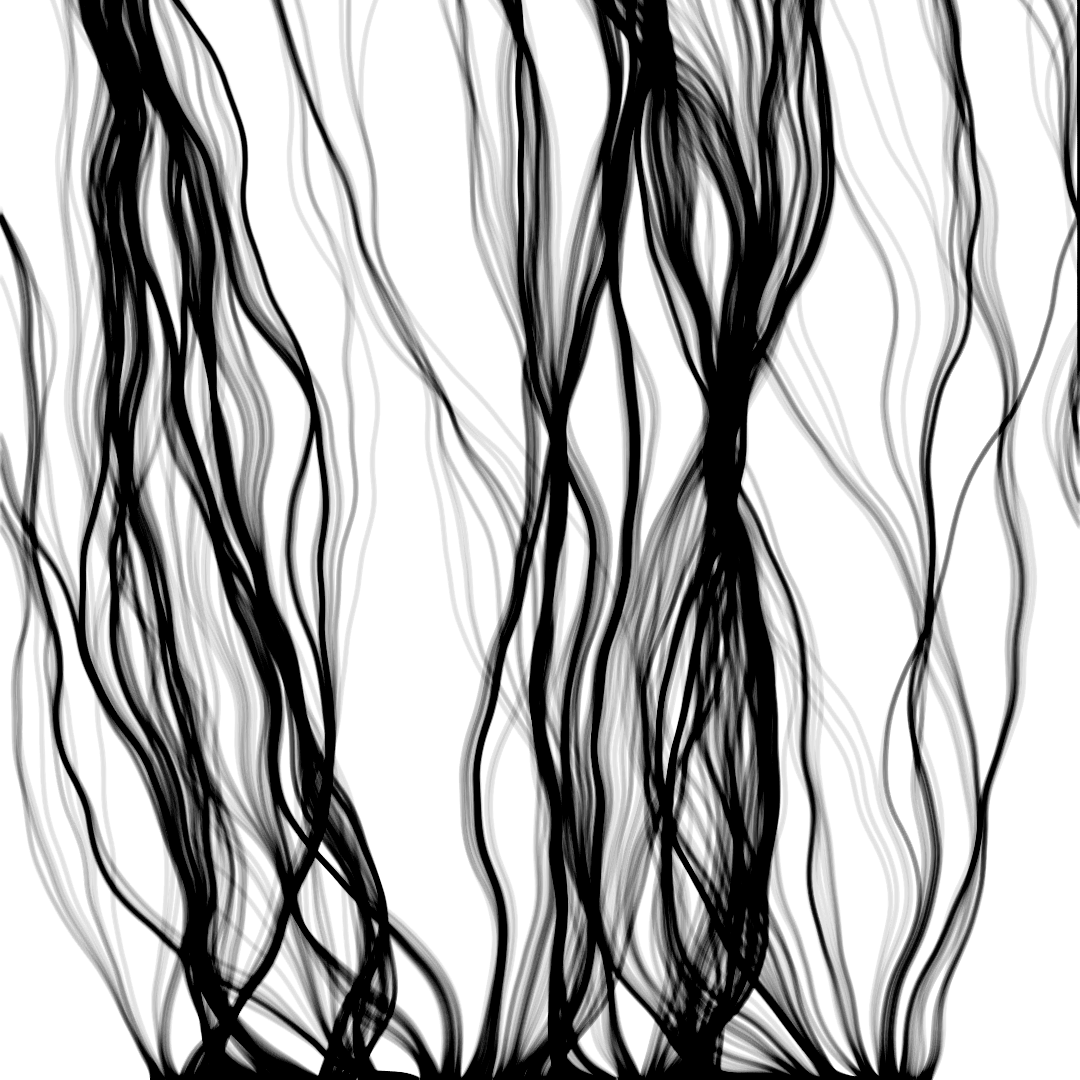
\includegraphics[scale=0.15]{images/cover}
}
\subtitle{}
\author[Dr. Johannes Riesterer] % (optional, for multiple authors)
{Dr.  rer. nat. Johannes Riesterer}

\date[KPT 2004] % (optional)
{}

\subject{Angewandte Mathematik}

\frame{\titlepage}






\begin{frame}
    \frametitle{Infinitessimalrechnung}
    \framesubtitle{Infinitessimalrechnung}
    \begin{block}{Sir Isaac Newton}
\begin{figure}[H]
      \centering
    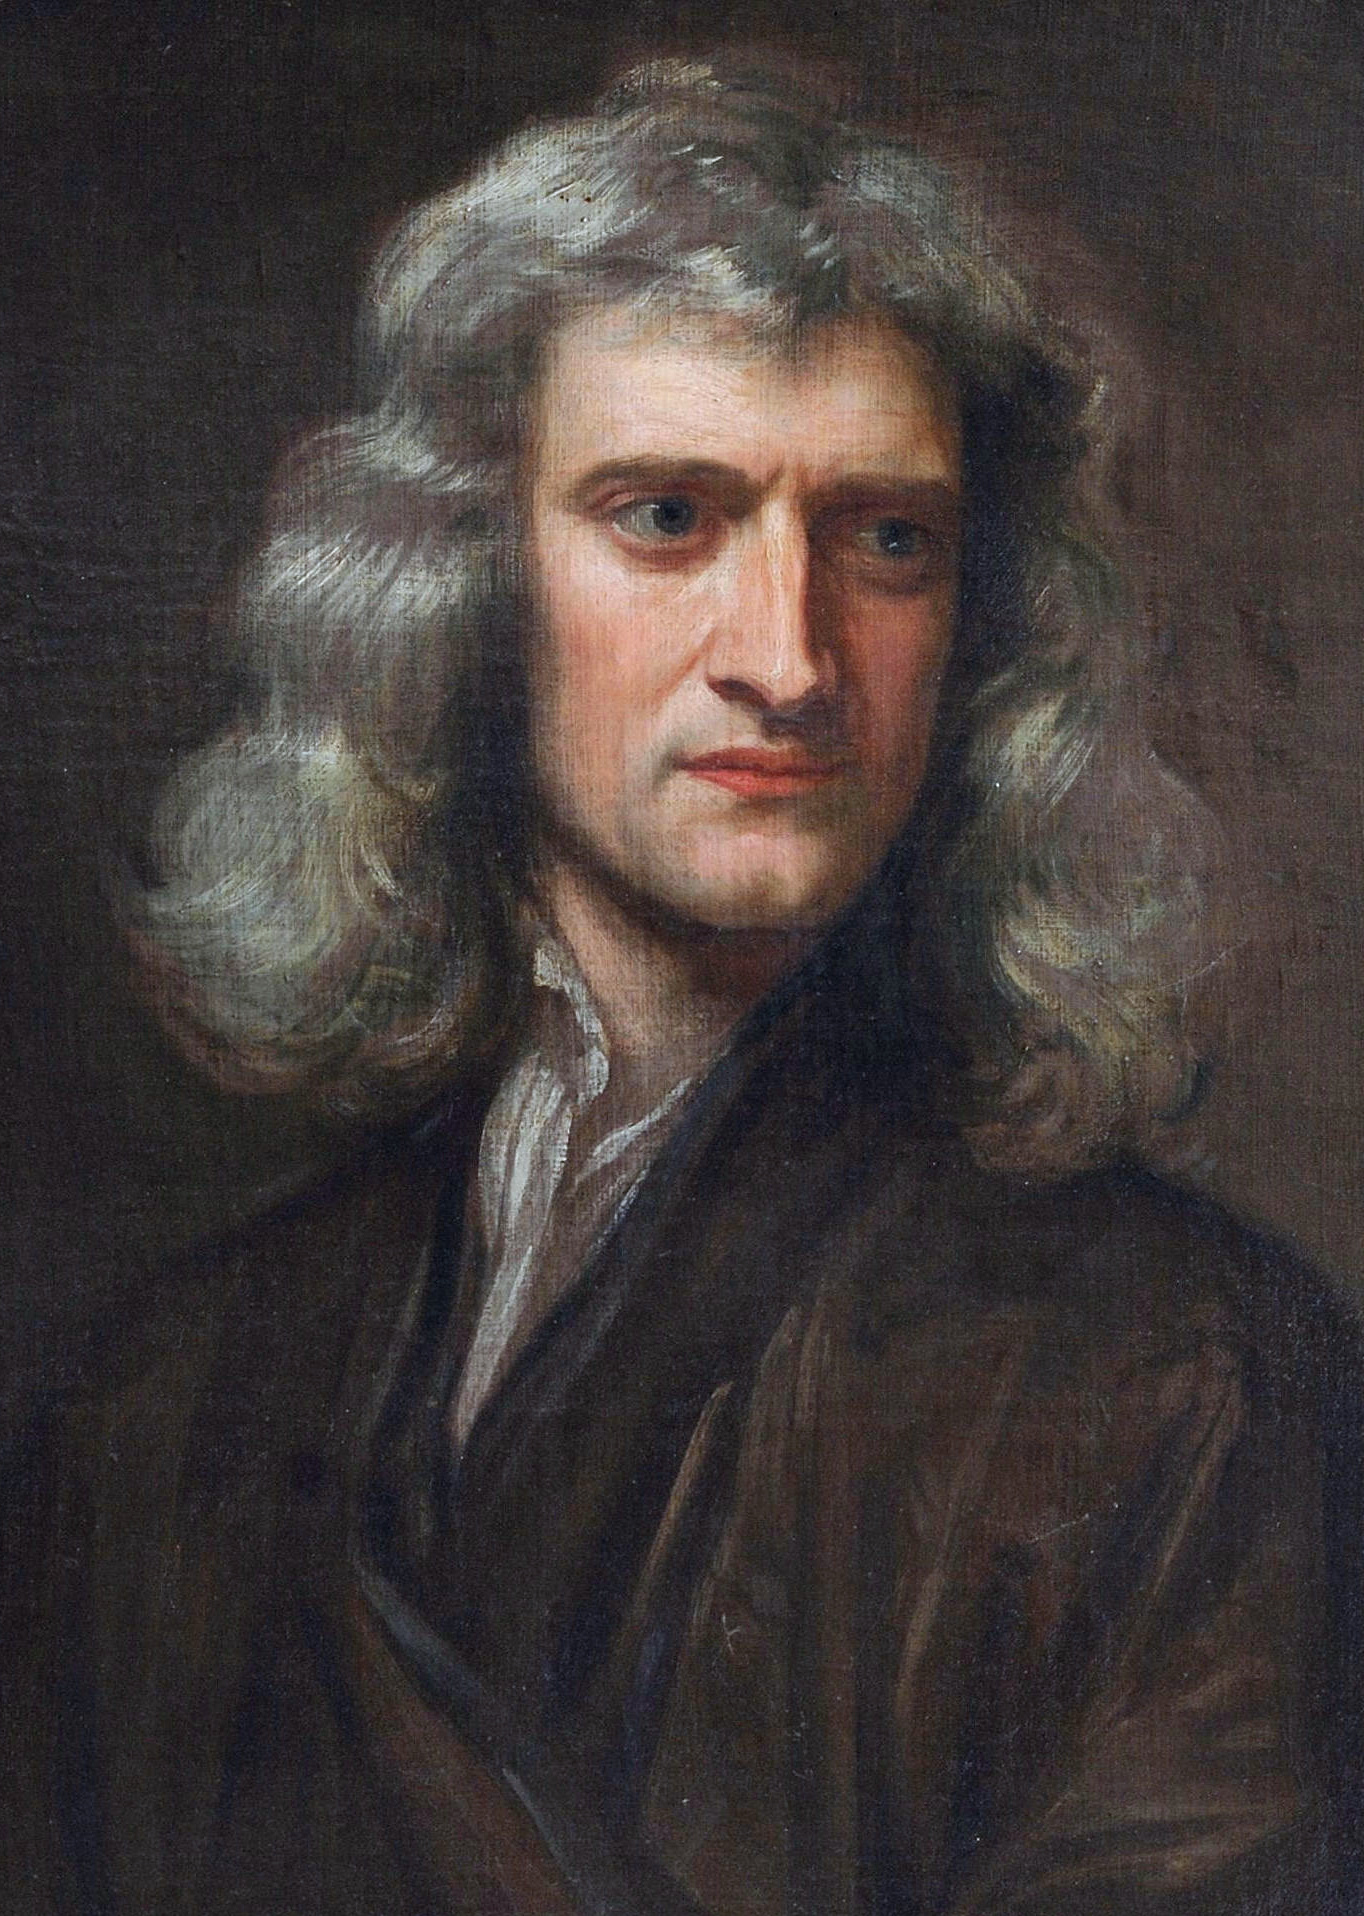
\includegraphics[width=0.6\textwidth]{images/Newton.jpg}
      \caption{Quelle: DALLE}
\end{figure}

\end{block}

 \end{frame}




 \begin{frame}
    \frametitle{Infinitessimalrechnung}
\framesubtitle{Infinitessimalrechnung}
    \begin{block}{Konvergenz erfahrungsgemäß}
Etwas  konvergiert gegen einen Grenzwert, 
wenn es sich diesem Grenzwert beliebig nahe annähert.
\end{block}

    \begin{figure}[H]
          \centering
        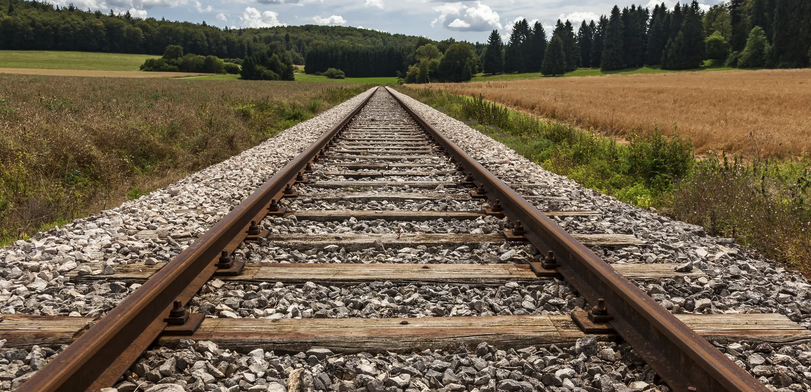
\includegraphics[width=0.8\textwidth]{images/limit}
          \caption{Konvergente Schienen}
    \end{figure}

\end{frame}


\begin{frame}
    \frametitle{Infinitessimalrechnung}
\framesubtitle{Infinitessimalrechnung}
    \begin{block}{Infinitessimalrechnung}
        Wie kann man damit rechnen und braucht man das?
\end{block}
 \end{frame}


 \begin{frame}
    \frametitle{Infinitessimalrechnung}
\framesubtitle{Limes}
    \begin{block}{Achilles und die Schildkröte}
\begin{figure}[H]
      \centering
    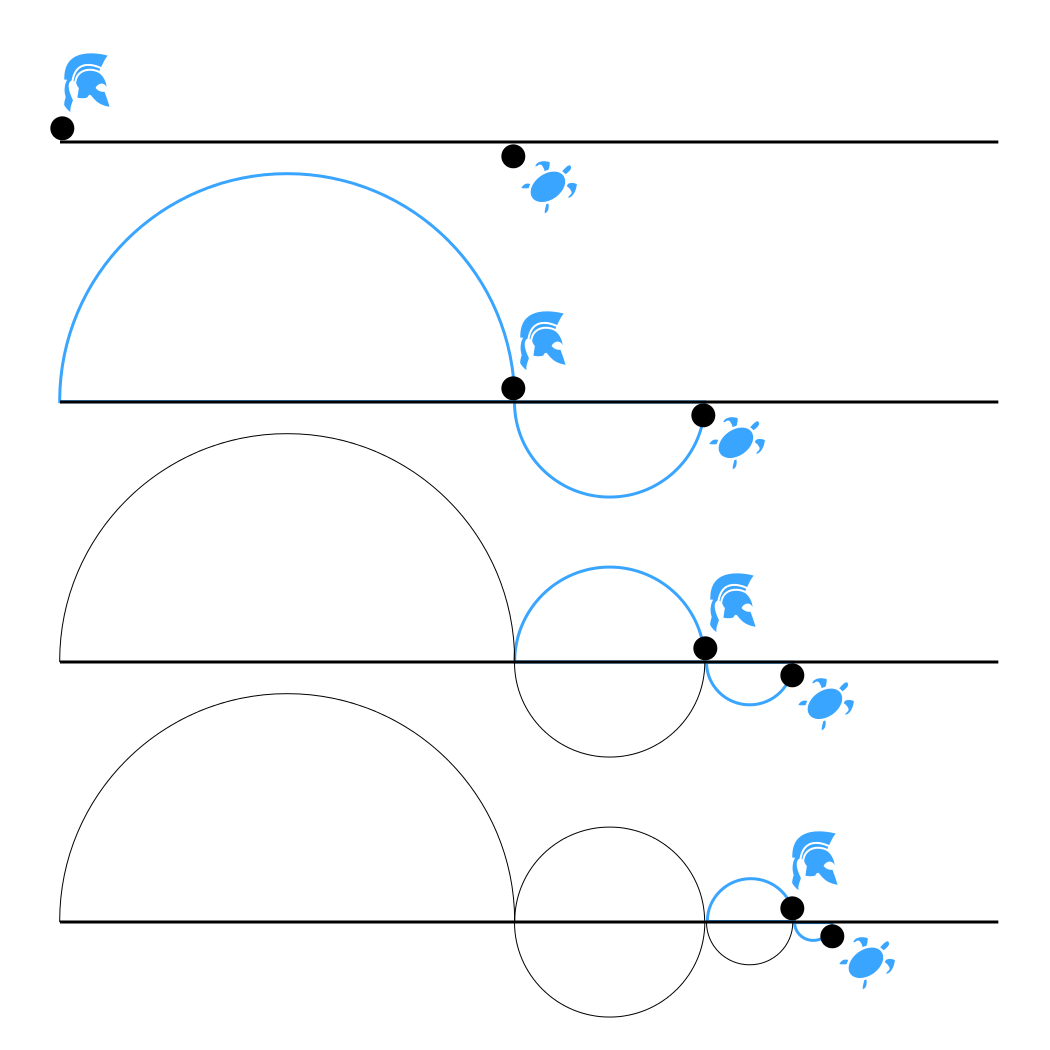
\includegraphics[width=0.3\textwidth]{images/Zeno_Achilles_Paradox}
      \caption{Quelle: Wikipedia: }
\end{figure}
\href{https://www.youtube.com/watch?v=X8Qksx_Ng9k}{Mehr hier im Video}
\end{block}
  \begin{block}{Paradoxon der Antike}
 Obwohl Achilles schneller ist, kann er die Schildkröte niemals einholen.
\end{block}
 \end{frame}


\begin{frame}
    \frametitle{Infinitessimalrechnung}
\framesubtitle{Limes}
    \begin{block}{Achilles und die Schildkröte infinitessimal betrachtet}
Sei $s_0$ der Vorsprung der Schildkröte zu Beginn des Rennens, $t_0$ die Zeit, die Achilles benötigt, um $s_0$ zurückzulegen. Die Schildkröte ist $q$-mal langsamer als Achilles.
Dann holt Achilles die Schildkröte nach der Zeit $t_0 \cdot q$ ein weiteres Mal ein, nach der Zeit $(t_0 \cdot q) \cdot q = t_0 \cdot q^2$ ein drittes Mal usw.
Mit $q^0 = 1$ ist die Summe aller betrachteten Zeiten, die Achilles zurücklegt:

$t = t_0 \cdot \sum_{n=0}^\infty q^n = t_0 \cdot \lim_{n \to \infty} \sum_{k=0}^{n} q^{k} = t_0 \cdot \lim_{n \to \infty} \frac{1 - q^{n+1}}{1 -q} = \frac{t_0}{1 -q}$.
\end{block}
 \end{frame}






\begin{frame}
    \frametitle{Infinitessimalrechnung}
\framesubtitle{Limes}

\begin{block}{Folge}
    Eine reelle Folge ist eine Abbildung
    \begin{align*}
    a: \mathbb{N} \rightarrow \mathbb{R}^n
    \end{align*}
 Für $n \in \mathbb{N}$ bezeichnen wir $a_n := a(n)$ als $n$ tes Folgenglied.
\end{block}


 \end{frame}



 \begin{frame}
    \frametitle{Infinitessimalrechnung}
\framesubtitle{Limes}

\begin{block}{Konvergenz}
    Eine Folge $a_n$ in $\mathbb{R}^n$ heißt konvergent gegen den Grenzwert $a \in \mathbb{R}^n$, wenn gilt:
    \begin{align*}
    \forall {\varepsilon > 0} \ \exists \ N \in \mathbb{N} \; \forall \ n > N: \; d(a, a_n) < \varepsilon\,
    \end{align*}
    in Worten: Es gibt für jedes beliebige (noch so kleine) $\varepsilon$ einen Index $N$ derart, dass für alle Indizes $n > N$, alle weiteren Folgenglieder, gilt: der Abstand $d(a, a_n)$ ist kleiner als $\varepsilon$.
    \end{block}


\begin{figure}[H]
      \centering
    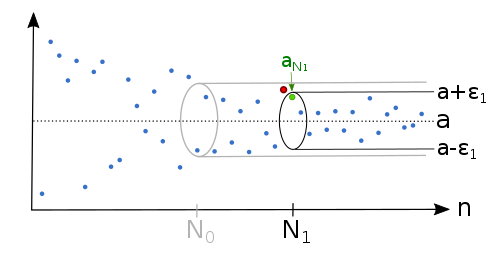
\includegraphics[width=0.7\textwidth]{images/500px-Epsilonschlauch_klein}
      \caption{Quelle: Wikipedia: https://commons.wikimedia.org/wiki/File:Epsilonschlauch\_klein.svg}
\end{figure}



 \end{frame}





\end{document}

